%% The first command in your LaTeX source must be the \documentclass command.
%%
%% Options:
%% twocolumn : Two column layout.
%% hf: enable header and footer.
\documentclass[
% twocolumn,
hf,
]{confart}

%%
%% One can fix some overfulls
\sloppy

%%
%% Minted listings support 
%% Need pygment <http://pygments.org/> <http://pypi.python.org/pypi/Pygments>
\usepackage{listings}
\usepackage{booktabs}
\usepackage{tabularx}
\usepackage{xcolor}
\definecolor{codegreen}{rgb}{0,0.6,0}
\definecolor{codegray}{rgb}{0.5,0.5,0.5}
\definecolor{codepurple}{rgb}{0.58,0,0.82}
\definecolor{backcolour}{rgb}{0.95,0.95,0.92}
\lstdefinestyle{mystyle}{
    backgroundcolor=\color{backcolour},   
    commentstyle=\color{codegreen},
    keywordstyle=\color{magenta},
    numberstyle=\tiny\color{codegray},
    stringstyle=\color{codepurple},
    basicstyle=\ttfamily\footnotesize,
    breakatwhitespace=false,         
    breaklines=true,                 
    captionpos=b,                    
    keepspaces=true,                 
    numbers=left,                    
    numbersep=5pt,                  
    showspaces=false,                
    showstringspaces=false,
    showtabs=false,                  
    tabsize=2
}

\lstset{style=mystyle}
%% auto break lines
\lstset{breaklines=true}

%%
%% end of the preamble, start of the body of the document source.
\begin{document}

% Set conference header (optional - modify as needed)
\setConferenceHeader{Your Conference Name}


%%
%% Rights management information.
%% CC-BY is default license.
\copyrightyear{2023}
\copyrightclause{Copyright for this paper by its authors.
  Use permitted under Creative Commons License Attribution 4.0
  International (CC BY 4.0).}

%%
%% This command is for the conference information
\conference{Your Conference Name. Conference Proceedings, City, Country, Date Range, Year.}

%%
%% The "title" command
\title{Your Paper Title Here: A Template for Conference Submissions}

% \tnotemark[1]
\tnotetext[1]{You can use this document as the template for preparing your
  publication.}

%%
%% The "author" command and its associated commands are used to define
%% the authors and their affiliations.
\author[1]{Your Name}[%
email=your.email@institution.edu,
url=https://your.website.com,
]
\fnmark[1]

\author[1]{Second Author}[%
email=second.author@institution.edu,
url=https://second.website.com,
]
\cormark[1]
\fnmark[1]

\fnmark[1]
\address[1]{Your Institution,
  Your Address, City, Country}

%% Footnotes
\cortext[1]{Corresponding author.}
\fntext[1]{These authors contributed equally.}

%%
%% The abstract is a short summary of the work to be presented in the
%% article.
\begin{abstract}
  This is a template for conference paper submissions. Replace this abstract with a concise summary of your research work, methodology, key findings, and contributions. The abstract should typically be 150-300 words and provide readers with a clear understanding of your paper's main points without requiring them to read the full document. Include the problem you're addressing, your approach or methodology, key results, and the significance of your findings.
\end{abstract}

%%
%% Keywords. The author(s) should pick words that accurately describe
%% the work being presented. Separate the keywords with commas.
\begin{keywords}
  Keyword 1 \sep
  Keyword 2 \sep
  Keyword 3 \sep
  Keyword 4 \sep
  Keyword 5
\end{keywords}

%%
%% This command processes the author and affiliation and title
%% information and builds the first part of the formatted document.
% Ensure the internal sequence and conference name exist before building the title
% (some versions of the class assume these are declared).
\ExplSyntaxOn
% create sequence only if it doesn't already exist
\cs_if_free:cTF { g_conf_logonote_seq } { \seq_new:N \g_conf_logonote_seq } { }
\ExplSyntaxOff

\maketitle

\section{Introduction}

This is a template for conference paper submissions. You can use this document as a starting point for your own research paper. Replace this content with your actual research work.

\subsection{Background and Motivation}

Describe the background of your research area and the motivation for your work. Explain the problem you are addressing and why it is important.

\subsection{Research Question and Objectives}

Clearly state your research questions and objectives. What specific problems are you trying to solve? What are your main contributions?

\subsection{Subsections}

You can create subsections within your paper to organize your content better. Use the \texttt{subsection} command to create new subsections as needed.

\subsubsection{Subsubsection}
You can also create subsubsections for further organization. Use the \texttt{subsubsection} command as needed.

\subsection{Adding Code Snippets}
Code snippets can be included in your paper using the \texttt{listings} package, for example Listing~\ref{lst:example_code}.

\begin{lstlisting}[language=Python, caption={An example Python code snippet.}, label={lst:example_code}]
def example_function():
    print("Hello, World!")
example_function()
\end{lstlisting}

\subsection{Adding Lists}
You can create lists using the itemize or enumerate environments.

\begin{itemize}
\item Item 1
\item Item 2
\item Item 3
\end{itemize}

\begin{enumerate}
\item Item 1
\item Item 2
\item Item 3
\end{enumerate}


\subsection{Adding Figures and Tables}
Include figures and tables to illustrate your points. You can label them and refer to them in the text, for example Figure~\ref{fig:example} and Table~\ref{tab:example_results}.

\begin{table}[htbp]
\centering
\renewcommand{\arraystretch}{0.8}
\begin{tabularx}{\columnwidth}{l*{4}{>{\centering\arraybackslash}X}}
\toprule
\textbf{Method} & \textbf{Parameter 1} & \textbf{Parameter 2} & \textbf{Accuracy (\%)} & \textbf{Time (ms)} \\
\midrule
Baseline & 10 & A & 85.2 & 120.5 \\
Method A & 15 & B & 89.7 & 95.3 \\
Method B & 20 & A & 92.1 & 110.8 \\
Method C & 25 & C & 94.6 & 88.2 \\
Proposed & 30 & B & 96.3 & 75.1 \\
\bottomrule
\end{tabularx}
\caption{Comparison of different methods and their performance metrics.}
\label{tab:example_results}
\end{table}


\begin{figure}[htbp]
    \centering
    % Replace 'example-image' with your actual image file
    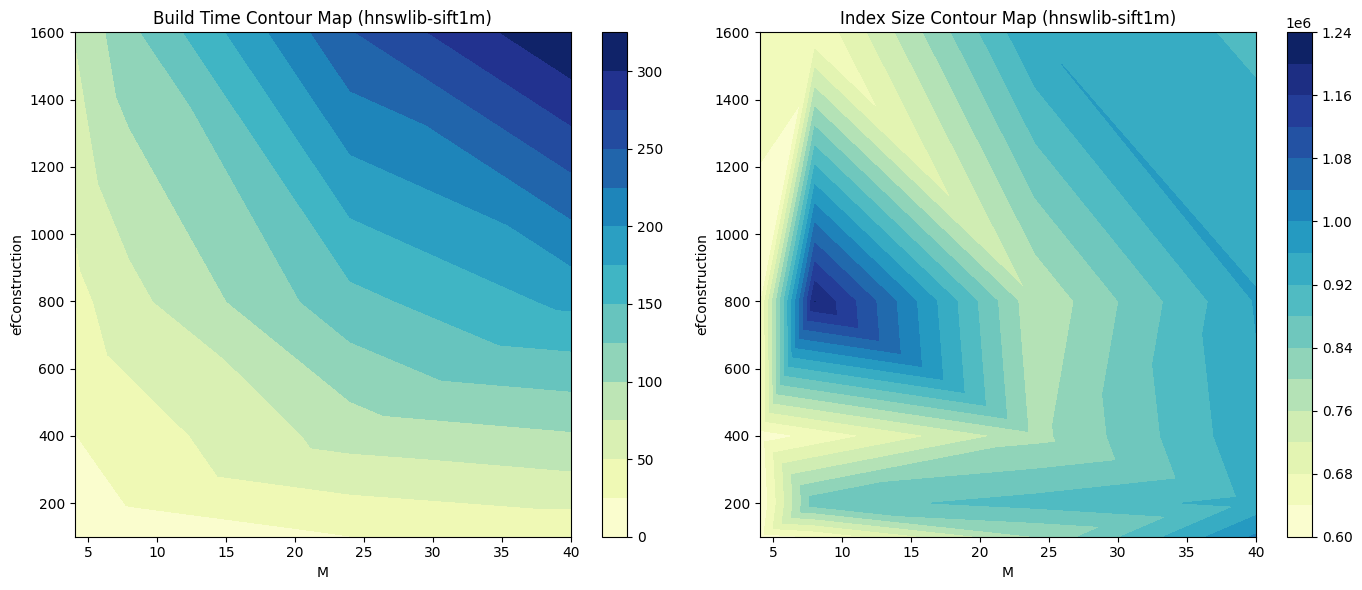
\includegraphics[width=0.5\textwidth]{assets/example.png}
    \caption{An example figure.}
    \label{fig:example}
\end{figure}

\subsection{Adding Citations}
You can add citations to your paper using the \texttt{bibtex} format. For example, you can cite a reference like this~\cite{guttman1984rtrees}. Make sure to include your bibliography file (e.g., \texttt{references.bib}) at the end of your document.


\subsection{Adding Appendix}
You can add an appendix section at the end of your paper using the \texttt{appendix} command. This is useful for including supplementary material, additional data, or detailed explanations that support your main content. In your writing, you can reference the appendix sections as needed like this (see Appendix~\ref{sec:appendix}).

%%
%% The acknowledgments section is defined using the "acknowledgments" environment
%% (and NOT an unnumbered section). This ensures the proper
%% identification of the section in the article metadata, and the
%% consistent spelling of the heading.
\begin{acknowledgments}
    This work is supported by\ldots
\end{acknowledgments}

%%
%% Define the bibliography file to be used (trimmed to only cited entries)
\bibliography{references}

%%
%% If your work has an appendix, this is the place to put it.
\appendix
\section{Appendix: Various Results}
\label{sec:appendix}
You can include additional results, data, or explanations in the appendix. This section is useful for providing supplementary information that supports your main content but is not essential to the primary narrative of your paper.

\end{document}

%%
%% End of file
